
%%%%%%%%%%%%%%%%%%%%%%%%%%%%%%%%%%%%%%%%%%%%%%%%%
%% 1. INTRODUCTION
%%%%%%%%%%%%%%%%%%%%%%%%%%%%%%%%%%%%%%%%%%%%%%%%%
% \section{Introduction}

Global optimization of multimodal and non-differentiable objective functions continues to
be an open research topic in the field of numerical optimization. Traditional
numerical techniques, such as linear programming and the simplex
method, have been applied with great success to linearly constrained objective functions
\cite{dantzig_linear_1997}. However, for certain types of problems they have been shown to
determine suboptimal solutions \cite{sarker_evolutionary_2002}. Also, when  linear
programming techniques are applied to multimodal performance surfaces, constraints must
be selected according to detailed knowledge of the performance surface topology. On the
other hand, genetic algorithms, which are a class of optimization algorithms that are
loosely based on the principles of evolution and genetics, have successfully determined
globally optimal solutions of multimodal and non-differentiable objective functions for
which linear programming algorithms could not determine the global optimum
\cite{fogel_what_2000}. Genetic algorithms  search a solution space by using genetic
operators and cumulative information to reduce a solution space and generate a
set of viable solutions. Some more recent genetic algorithms use orthogonal
crossover operators and have been shown to perform remarkably well for classical
challenging problems \cite{li_genetic_2006}. In this chapter a new algorithm called a
hybrid orthogonal genetic (HOG) algorithm that uses customized genetic operators to
improve algorithm performance and accuracy is applied to multimodal, non-differentiable
performance surfaces.

\section{Genetic Algorithms}
Figure 1 illustrates the flow chart of a typical genetic algorithm (GA). In GAs, a
population is defined as a set of $N$ individuals where individuals represent
possible solutions. At the outset, the population of $N$ individuals is initialized and
represents the first generation, denoted $G_0$, of the population's existence. If the
solution space topology is unknown, the rationale of the genetic algorithm is referred to
as an exploratory effort. Conversely, if the solution is known to exist in a localized
area of the solution space, the rationale is referred to as an exploitative effort. For
exploration of the performance surface, it is common to initialize the population with
individuals whose elements, characteristics, or traits, are uniformly distributed over the
solution space. However, to exploit localized areas of the performance surface, the
population is initialized with individuals whose traits are known to be near
optimal within some acceptable range of misadjustment.

\begin{figure}[htpb]
	\centering
	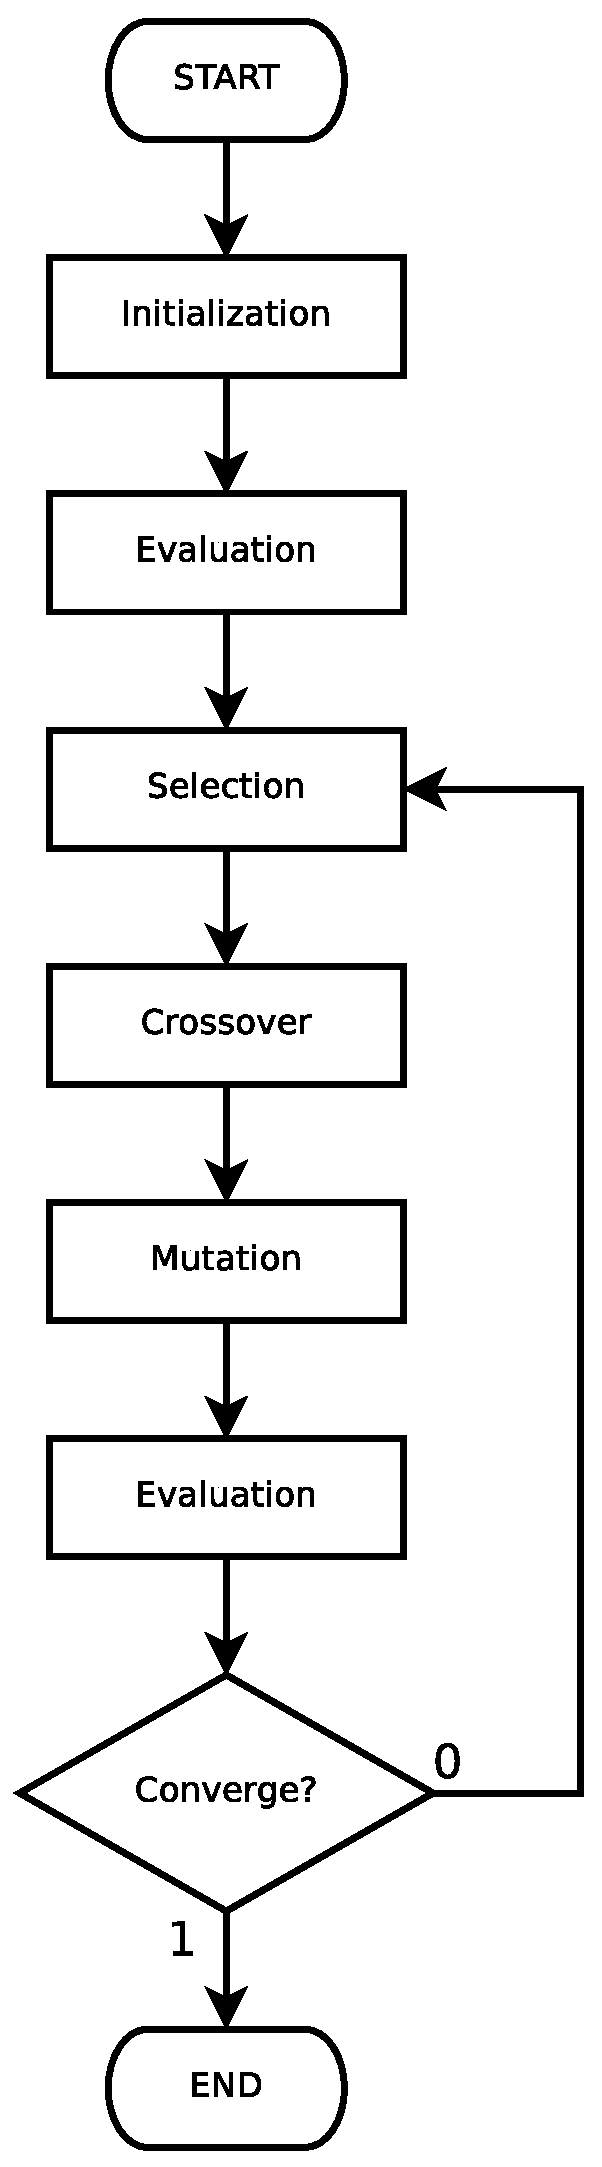
\includegraphics[height=0.65\textheight]{./figures/simple_ga_flow.eps}
	\caption{Traditional Genetic Algorithm Flow Chart}
	\label{fig:simple_GA_flow}
\end{figure}

Subsequent to initialization, each member of the population is evaluated by the
objective function, which is a metric of solution quality or fitness. Thus, an
individual's fitness is represented by the value, or cost, returned by the objective
function evaluation. Individuals are then selected according to their relative fitness for
placement into a mating pool which is a subset of the population. Individuals with a
higher relative fitness have a higher likelihood of selection for mating eligibility while
individuals with a lower relative fitness are more likely to be discarded. Individuals
which have been selected and placed into the mating pool then reproduce via a
crossover operator where reproduction is defined as the random exchange of traits between
selected individuals (progenitors) who produce offspring (progeny) and the crossover
operator is the algorithmic mechanism by which reproduction occurs. Following
reproduction, genetic diversity of the population is generated by introducing new
genetic information into the population via a mutation operator where mutation is defined
as the random alteration of a selected individual's traits.

Each member of the new population, $G_1$, which is now comprised of the mating pool and
their newly generated offspring, is evaluated for fitness. The new generation's
fitness is then analyzed to see if the convergence criteria has been met. If the
convergence criteria has not been met then the population must undergo
selection, reproduction, and mutation again and be reevaluated for convergence. This cycle
continues until the convergence criteria has been met.

%%%%%%%%%%%%%%%%%%%%%%%%%%%%%%%%%%%%%%%%%%%%%%%%
%% 2. HOG algorithm 
%%%%%%%%%%%%%%%%%%%%%%%%%%%%%%%%%%%%%%%%%%%%%%%%%
\section{Hybrid Orthogonal Genetic (HOG) Algorithm}

Figure \ref{fig:HOGA_flow_chart} shows a flow chart of the HOG algorithm which begins by
initializing the population with a random selection of viable solutions, referred to as
individuals or chromosomes. Structurally, each chromosome is represented by a vector of
length $K$ where each element or allele of the vector represents a trait which can be
viewed as genetic information in the chromosome. A population of size
$N$ can be represented by aggregating the chromosomes into a $K\times N$
matrix. Following population initialization, each chromosome is evaluated for fitness
by the objective function. The chromosomes are then sorted and linearly ranked
according to their fitness and selected for placement into a mating pool
according to their relative fitness. Once selected for mating eligibility, pairs of
chromosomes reproduce via a traditional crossover operator producing a pair of offspring.
The offspring and mating pool then reproduce a second time via a hybrid orthogonal
crossover operator. Genetic diversity is then generated through the use of a
mutation operator. Finally, the new generation's fitness is evaluated and the
results are examined for convergence. If convergence conditions are not met then the
process repeats itself until the convergence conditions are satisfied.

\begin{figure}[htbp]
	\centering
	\includegraphics[width=0.9\textwidth]{./figures/HOGA_flow.eps}
	\caption{Hybrid Orthogonal Genetic Algorithm Flow Chart}
	\label{fig:HOGA_flow_chart}
\end{figure}

\subsection{Population Initialization}
In the HOG algorithm, the initial population can be chosen such that the chromosomes are
uniformly distributed over some subset of the solution space. Typically, the initial
population is determined by the nature of the objective function. If the boundaries of
the objective function's feasible solution space are well understood then the initial
population can be selected over the known subset of this feasible solution space.
However, if the boundaries of the feasible solution space are unknown or poorly understood
then it may become necessary to iteratively modify the problem space as knowledge of the
performance surface is gained through trial and error.

\subsection{Fitness Evaluation}
As mentioned previously, the fitness of an individual is determined by evaluating the
objective function for that individual.  Because the HOG algorithm is a minimization based
evolutionary strategy, individuals with lower cost are considered more fit than
individuals with a higher cost. Thus, the HOG algorithm is searching for the individual
$\mathbf{x}$ that satisfies 
%---------------------
\begin{equation}\label{eq:objective_function}
\min_{\mathbf{x}\in\mathbb R^K}\bigl\{J(\mathbf{x})\bigr\}, \quad\mathbf{x}\in S
\end{equation}
%---------------------
where $J(\mathbf{x})$ is the cost or objective function,  $\mathbf{x}$ is a real vector in
$\mathbb{R}^K$, and $S$ is the set of feasible solutions.

\subsection{Linear-Ranking Selection}
 After the individuals in the population are linearly ranked according to their fitness,
each individual is assigned a probability of selection for reproduction such that more fit
individuals have a higher likelihood of reproducing than less fit individuals.
Individuals not selected for reproduction are discarded. In this thesis, the individual
with the best fitness is always selected for mating eligibility ensuring that the most fit
member of any generation is eligible for reproduction. Such algorithms are referred to as
elitist algorithms where elitist is defined as preserving the most fit individual for the
next generation independent from the evolutionary process. The HOG algorithm implements an
elitist, linear-ranking selection scheme to decrease stochastic selection variability and
improve the representation of highly dynamic populations for mating eligibility.

In biological terms, the genotype of a population is defined as the total available
genetic information belonging to that population. The phenotype of a population is defined
as the expressed traits of the population where expression is defined as the observable
display of characteristics related to a particular genetic composition. In evolutionary
systems, phenotypic expression and genotypic content are often very loosely coupled and
extremely difficult to characterize. As such, the observed fitness of an individual
belonging to some population offers only a partial indication of possible reproductive
optimality. Care must be taken that the evolutionary process does not inadvertently
discard the genetic information contained in less-fit individuals which may be required to
achieve the optimal chromosome. Prior to convergence, the optimal chromosome typically
exists as some permutation of traits belonging to individuals which cannot be guaranteed
to have the highest relative fitness. In fact, population dynamics typically exist such
that the relative difference between the most fit and least fit individual is poorly
reflected in its observed fitness even for well formed objective functions
\cite{blickle_comparison_1996}. As such, for most objective functions, the fitness metric
is not a good metric for determining an individual's breeding potential.

To mitigate the statistical selection bias inherent to the objective function, a linear
ranking scheme can be implemented where the population is ordered according to its fitness
prior to selection for mating eligibility \cite{whitley_genitor_89}. In the HOG algorithm,
the population of $N$ individuals is sorted according to their fitness values. Once
sorted, the individuals from the least fit (highest cost) to most fit (lowest cost)
are assigned consecutive integers from 1 to $N$; that is, the least fit individual is
assigned one and the most fit individual is assigned $N$. The probability of selection for
mating eligibility is then assigned according to the individual's rank within the
greater population where the $i$th ranked individual has the probability, $p_i$, of
selection, given as
%---------------------
\begin{equation}\label{eq:linear_ranking}
p_{i}=\frac{1}{N}\biggl(\eta^{-}+\bigl(\eta^{+}-\eta^{-}\bigr)\frac{i-1}{N-1}\biggr)
\end{equation}
%---------------------
where $\bigl(\eta^{-}/N\bigr)$ and $\bigl(\eta^{+}/N\bigr)$ are the probabilities of
selection for the least fit and most fit individual, respectively.
Because the population is comprised of $N$ disjoint elementary events,
%---------------------
\begin{equation}\label{eq:linear_ranking_pdf}
\sum_{i=1}^{N}p_{i}=\sum_{i=1}^{N}\frac{1}{N}\biggl(\eta^{-}+\bigl(\eta^{+}-\eta^{-}
\bigr)\frac{i-1}{N-1}\biggr) = 1\text{.}
\end{equation}
%---------------------
which implies that $\eta^{-}=2-\eta^{+}$ where $0\leq\eta^{+}\leq2$.

Specific selection of $\eta^{-}$ and $\eta^{+}$ allows for control over selection pressure
which is defined as the relationship between the probability of selection of the most fit
vs. least fit individual. It has been shown that fixing $\eta^{+}$ at 1.1 provides an
adequate balance between exploration and exploitation of the performance surface
\cite{back_optimization_1991}.

Because standard operators which rely on stochastic selection where the
probability of selection is proportional to the individual's relative fitness cannot
guarantee that the most fit individuals will be considered for selection and subsequent
reproduction, the possibility exists that good chromosomes may be randomly
discarded. For the HOG algorithm, an elitist selection method is implemented to counter
this phenomenon, where elitism is defined as the process of automatically selecting the
best chromosome(s) for mating eligibility thereby ensuring the availability of their
genetic information for subsequent reproduction. This technique has been shown to greatly
increase convergence speeds, especially for applications where minimizing steady-state
misadjustment is significant \begin{large}                            
\end{large}\cite{reeves_genetic_2002}.

\subsection{Single Point Crossover}
After randomly selecting a group of eligible progenitors, or a mating pool, using the
selection probabilities, randomly paired individuals reproduce by exchanging alleles
where alleles are the elements comprising the vector structure of the chromosome. In
genetic algorithms, this process is referred to as crossover. This sharing of genetic
information is the vehicle by which individuals propagate their beneficial traits.

For both single-point and hybrid orthogonal crossover, pairs of progenitors are randomly
selected from the mating pool and are given the opportunity to exchange genetic
information via the respective crossover operator. Each selected pair is assigned a random
number, $r$ that has a uniform distribution over $\bigl[0,1\bigr]$. Selection for
crossover is governed by the coefficient for crossover probability of, $P_c$, which
typically ranges from 0.2 to 1.0. If $r<P_c$, crossover occurs and genetic information is
exchanged between the pair of progenitors and offspring are produced. Conversely, if
$r\geq P_c$, the pair is returned to the mating pool without producing offspring. Note
that the process by which individuals are randomly selected for crossover is typically
regulated. For this application, self replication is strictly forbidden. Thus,
selected individuals must crossover with a different individual thereby ensuring the
exchange of alleles and preventing a single anomalous individual from inadvertently
dominating the greater population leading the algorithm to converge to a non-optimal
solution.

Recall that reproduction is defined as the exchange of genetic information
between two individuals belonging to a population and that the mechanism of exchange of
vector elements between the individuals is referred to as the crossover operator. Many
different crossover techniques have been analyzed and implemented successfully across a
broad range of objective function types
\cite{poon_genetic_1995}\cite{glover_handbook_2003}. Because the objective function both
characterizes the problem space and evaluates specific chromosomes, the physical structure
of the chromosomes is determined by the characteristics of the objective function.
Thus, the optimal crossover operator is related to the physical structure of the
chromosome. For certain applications, it may be necessary to regulate which alleles can be
exchanged. These regulations are dictated by the relationships which exist between
adjacent groups of alleles. The power of evolutionary strategies lies in achieving a
balance between exploring a solution space and exploiting its localized minima or maxima.
As a result, a balance between preserving the stochastic nature of reproduction and the 
deterministic exchange of genetic information must be maintained. Thus, the
structure of the chromosome should complement the crossover method selected. For the
HOG algorithm, reproduction is achieved by using both a single-point crossover operator
and a hybrid orthogonal crossover operator based on the Taguchi method.

The single-point crossover operator is an arithmetic operator derived from convex set
theory which randomly selects a single crossover point for the selected chromosomes
\cite{jinn-tsong_tsai_hybrid_2004}. For two individuals represented by the real
vectors $\mathcal{C}_\alpha$ and $\mathcal{C}_\beta$, all alleles subsequent to the
crossover point are exchanged between the progenitors and two progeny are created. The
single-point crossover process is illustrated in Figure \ref{fig:crossover} where the
progenitor chromosomes are denoted as $\mathcal{C}_\alpha$ and $\mathcal{C}_\beta$ and the
progeny chromosomes are denoted as $\mathcal{C}_\alpha^\prime$ and
$\mathcal{C}_\beta^\prime$.
%----------------------------
\begin{figure}[H]
\centering
\includegraphics[width=\textwidth]{./figures/crossover.eps}
\caption{Single-Point Crossover}
\label{fig:crossover}
\end{figure}
%----------------------------
Single-point crossover has positional bias in that it favors continuous segments of
genetic information. However, it does not contain distribution bias as the crossover
point  is a discrete random variable with uniform distribution over $\bigl[0,m\bigr]$,
where $m$ denotes the length of the respective chromosome \cite{glover_handbook_2003}.

%%%%%%%%%%%%%%%%%%%%%%%%%%%%%%%%%%%%%%%%%%%%%%%%%%%%%%%%%%%%%%%%%%%%%%%%%%%%%%%%
\subsection{Hybrid Orthogonal Crossover via The Taguchi Method}
After traditional single-point crossover has been performed, the previously selected
mating pool and newly generated progeny undergo an additional exchange of genetic
information using a hybrid crossover technique which intelligently creates more fit
offspring. Unlike the traditional crossover operator, the hybrid orthogonal crossover
operator intelligently draws genetic information from each progenitor to create the best
possible offspring given the traits that are available. Based on the Taguchi method and
using orthogonal-array based experimental design techniques, this method has been shown
to produce the most robust offspring possible given the genetic information available from
the current population \cite{jinn-tsong_tsai_optimal_2006}. It has also been shown to be
significantly less sensitive to ill-formed objective functions and non-linear performance
surfaces and to improve both solution accuracy and overall convergence speed
\cite{jinn-tsong_tsai_hybrid_2004}.

The progenitors are randomly selected from the eligible mating pool as is done 
for the traditional crossover operator. However, unlike traditional crossover operators,
all permutations of possible progeny for a selected pair of progenitors are considered
with the hybrid operator. Each permutation of genetic exchange between the progenitors is
treated as an experiment (trial) where the factors of the experiment correspond to the
available traits. The subsequent fitness evaluation of the progeny can then be treated as
the observation of an experimental trial of $K$ factors where $K$ is
the length of each chromosome
\cite{yiu-wing_leung_orthogonal_2001}\cite{jinn-tsong_tsai_hybrid_2004}. This type of
experiment is commonly referred to as a factorial experiment of $K$ factors. As such,
proven methods from the statistical design of experiments can be used to improve
the experimental process. Specifically, statistical design of experiments is the process
of planning experiments so that significant data can be collected with a minimum number
of performed experiments. Subsequent to data collection, suitable statistical methods are
then used to analyze the collected data and draw statistical inferences accordingly
\cite{shinn-ying_ho_intelligent_2004}.

%%%%%%%%%%%%%%%%%%%%%%%%%%%%%%%%%%%%%%%%%%%%%%%%%%%%%%%%%%%%%%%%%%%%%%%%%%%%%%%%
\subsubsection{Design of Experiments and Orthogonal Arrays}
For a factorial experiment of $K$ factors, there exists $N^K$ trials where $N$ represents
the number of levels for each factor. For the hybrid orthogonal crossover operator, $N=2$
because only two progenitors are available from which to draw traits. Thus, $2^K$
experiments must be performed to determine the most optimal progeny from the
full factorial experiment space where $K$ corresponds to the number of traits
 or experimental factors. Because each permutation must be evaluated by the objective
function to determine the experimental results for that particular trial, performing
all $2^K$ objective function evaluations becomes computationally prohibitive for large
values of $K$. As such, fractional factorial design of experiments can be used to reduce
the number of required experimental trials. The HOG algorithm uses orthogonal array based
design of experiments to reduce the full factorial solution space to a small but
representative number of sample trials\cite{yiu-wing_leung_orthogonal_2001}.

The Taguchi method of design of experiments utilizes two-level orthogonal arrays which are
special arrays derived from the Latin square. An $M$ row and $N$ column Latin square,
denoted as $L_M$, has the form
%---------------------------
\begin{equation}\label{eq:latin_array}
L_{M}\bigl(Q^{N}\bigr) = \bigl[a_{i,j}\bigr]_{M\times
N},\quad a_{i,j}\in\{1,2,\cdots,Q\}
\end{equation}
%---------------------------
where the $M$ rows represent the experimental trials, the $N$ columns
represent the experimental factors, and $Q$ corresponds to the number of levels of
the experimental design\cite{yiu-wing_leung_orthogonal_2001}. Recall that the
hybrid orthogonal crossover operator uses two-level orthogonal arrays. As
such, substituting $Q=2$ into \eqref{eq:latin_array} yields 
%---------------------------
\begin{equation}\label{eq:two_level_array}
L_n\bigl(2^{n-1}\bigr)
\end{equation}
%---------------------------
where $n$ corresponds to the number of trials. The resulting Latin square then represents
an orthogonal set of experiments where orthogonal is defined as the statistical
independence of the columns representing experimental factors. The observations
made over $n$ trials of orthogonal experiments yields the effects of the experimental
factors. In particular, the HOG algorithm uses this information to determine which factors
have the most beneficial contribution to the progeny.

To illustrate, consider an experiment that has 3 factors (alleles) and 2 levels
(progenitors). For this experiment, $2^3$, or 8, unique experiments exist in the full
factorial experiment space.  The Latin square which represents the experimental space is
given as 
%---------------------------
\begin{equation}\label{eq:two_level_array_example}
L_4\bigl(2^{3}\bigr)=
\begin{pmatrix}
1 &1 &1 \\
1 &2 &2 \\
2 &1 &2 \\
2 &2 &1 \\
\end{pmatrix}
\end{equation}
%---------------------------
 which is a 2-level orthogonal array of 4 trials. If the 2's in
\eqref{eq:two_level_array_example} are replaced with -1's, then the inner
product of any two columns of the experimental matrix is null indicating that all
columns of the orthogonal array are mutually orthogonal. Because the columns are
orthogonal the effect of any factor across all trials is statistically independent from
the effect of any other factor \cite{dean_design_2000}. To illustrate, consider 2
progenitors $\mathbf{\alpha}$ and $\mathbf{\beta}$ where $\bm{\alpha}=[ \alpha_1 \quad
\alpha_2 \quad \alpha_3 ]^T$ and $\bm{\beta}=[\beta_1 \quad \beta_2 \quad \beta_3 ]^T$.
Using \eqref{eq:two_level_array_example} to generate the orthogonal experimental matrix,
the corresponding experimental trials and factors are represented by the rows and columns
of Table \ref{tbl:alpha_beta_table} respectively.
%---------------------------
\begin{table}[htpb]
\caption{Two-Level Experimental Matrix for 3 Factors}\label{tbl:alpha_beta_table}
\begin{center}
\begin{tabular}{cccc}
\toprule
Trial ($n$) & \multicolumn{3}{c}{Factors}\\
\midrule
1 & $\alpha_1$ & $\alpha_2$ & $\alpha_3$ \\ 
2 & $\alpha_1$ & $\beta_2$ & $\beta_3$ \\ 
3 & $\beta_1$ & $\alpha_2$ & $\beta_3$ \\
4 & $\beta_1$ & $\beta_2$ & $\alpha_3$ \\ \bottomrule
\end{tabular}
\end{center}
\end{table}
%---------------------------

The Latin square and the full factorial experiment space can be represented
graphically as depicted in Figure \ref{fig:orthogonal_array_plot} where $\phi_x$ represent
the independent factors and the vertices correspond to the space-representative
trials.
%---------------------------
\begin{figure}[htbp]
\centering
\includegraphics[width=0.6\textwidth]{./figures/orth_array_plot.eps}
\caption{Graphical Representation of $L_{4}\bigl(2^3\bigr)$}
\label{fig:orthogonal_array_plot}
\end{figure}
%---------------------------
As illustrated in Figure \ref{fig:orthogonal_array_plot}, the edges of the graph enclose
the full factorial experiment space. On inspection, it is clear that the full factorial
space of 8 experiments has been reduced to the evaluation of a subset of 4 vertices
thereby decreasing the total number of trials necessary to observe the effects of
the experimental factors by a factor of two.

%%%%%%%%%%%%%%%%%%%%%%%%%%%%%%%%%%%%%%%%%%%%%%%%%%%%%%%%%%%%%%%%%%%%%%%%%%%%%%%%
\subsubsection{Taguchi Method}
To estimate an optimal set of alleles, or factors, from the reduced factorial experiment
space, the Taguchi method determines the cost of each trial of the experimental matrix
and processes these costs in a metric which is used to calculate the observed
effects of all available alleles. Based on this calculation, a set of alleles are selected
from the available progenitors to produce an estimated optimal progeny.

This thesis uses the metric $S_n$ which is defined as the cost
function squared for the $n$th trial, that is, 
%---------------------------
\begin{equation}\label{eq:MSE}
S_n=J^{2}(\bm{x}_n)
\end{equation}
%---------------------------
where $\bm{x}_n$ is a vector containing the alleles, or factors, of the $n$th trial. This
metric is then used to calculate each allele's observed effect which is subsequently
used for determining an estimated optimal progeny.

The observed effect, $E_{x_{k}P_{m}}$, for an allele or factor $x_k$ is defined as the sum
of the metrics, $S_n$, for which the $n$th trial corresponds to the $m$th progenitor's
factor contribution. For example, for the two-level experiment given in Table
\ref{tbl:alpha_beta_table}, the observed effect is given as 
%---------------------------
\begin{equation}\label{eq:effects_of_factors}
 E_{x_{k}P_{m}}=\sum_{i\in \{k:x_k = P_m\}}S_i
\end{equation}
%---------------------------
where $i$ corresponds to the trial number in which the $m$th progenitor $P_m$ contributed
its $k$th respective factor.  For a global minimizer, the optimal contributing $k$th
allele is defined as the allele from the progenitor which gives the lowest value for
$E_{x_{k}P_{m}}$. To illustrate, consider an experiment with two progenitors which
corresponds to a two-level orthogonal array. If $E_{x_{k}P_1} < E_{x_{k}P_2}$ for the
factor $x_k$, the optimal contribution is given by progenitor 1 ($P_1$). Conversely, for
$E_{x _{k}P_1} > E_{x_{k}P_2}$, progenitor 2 ($P_2$) would provide the optimal
contribution \cite{jinn-tsong_tsai_hybrid_2004}. The optimal chromosome is then assembled
by taking the factor from the optimal progenitor for each of the $K$ factors in the
chromosome. This process is further illustrated in the following example.

\subsubsection{Taguchi Method Example}
To illustrate the Taguchi method, consider a cost function $J(\bm{x})$ given as 
%---------------------------
\begin{equation}\label{eq:taguchi_ex_cost_fn}
J(\bm{x})=\sum_{i=1}^{7}x_i^2
\end{equation}
%---------------------------
where $x_1,x_2,\dots,x_7$ are real elements of the vector $\bm{x}$.
Equation \eqref{eq:taguchi_ex_cost_fn} describes an elliptic paraboloid that has a
global minimum at zero.
\sloppy
Consider two randomly selected progenitors, $\mathcal{C}_1$ and $\mathcal{C}_2$, where
$\mathcal{C}_1 = [1 \quad 1 \quad 1 \quad 1 \quad 0 \quad 0 \quad 0]$ and $\mathcal{C}_2 =
[0 \quad 0 \quad 0 \quad 0 \quad 1 \quad 1 \quad 1]$. Because the experiment has 7
factors, or alleles, and 2 progenitors, or levels, the orthogonal array,
$L_{8}\bigl(2^7\bigr)$, where 
%---------------------------
\begin{equation}\label{eq:taguchi_ex_orth_arry}
L_{8}\bigl(2^7\bigr)=
\begin{pmatrix}
1     &1     &1     &1     &1     &1     &1\\
1     &1     &1     &2     &2     &2     &2\\
1     &2     &2     &1     &1     &2     &2\\
1     &2     &2     &2     &2     &1     &1\\
2     &1     &2     &1     &2     &1     &2\\
2     &1     &2     &2     &1     &2     &1\\
2     &2     &1    &1     &2     &2     &1\\
2     &2    &1     &2     &1     &1     &2\\
\end{pmatrix}
\end{equation}
%---------------------------
can be used to form an appropriate experimental matrix. Using the orthogonal array shown
in \eqref{eq:taguchi_ex_orth_arry}, the experimental matrix illustrated in Table
\ref{tbl:taguchi_ex_table} can be created where $n$ denotes the trial number,
$x_k$ denotes the $k$th experimental factor, $\bm{x}_n$ represents the chromosome for
the $n$th trial, $J(\bm{x}_n)$ corresponds to the evaluated cost for the $n$th
experimental trial, and $S_n$ corresponds to the calculated metric for the $n$th
experimental trial.
%---------------------------
\begin{table}[htbp]
\begin{center}
 \caption{Taguchi Method Example Experimental Matrix}\label{tbl:taguchi_ex_table}
 \begin{tabular}{ccccccccccc}\toprule
\multirow{2}*{Trial ($n$)} &
\multirow{2}*{Chromosome} &
\multicolumn{7}{c}{Experimental Factors} & 
\multirow{2}*{$J_{n}(\bm{x}_n)$} &
\multirow{2}*{$S_n$} \\ 
&
&
$x_1$ &
$x_2$ &
$x_3$ &
$x_4$ &
$x_5$ &
$x_6$ &
$x_7$ & \\ \midrule 
1 & $\bm{x}_1$ & 1 & 1 & 1 & 1 & 0 & 0 & 0 & 4 & 16 \\ 
2 & $\bm{x}_2$ & 1 & 1 & 1 & 0 & 1 & 1 & 1 & 6 & 36\\ 
3 & $\bm{x}_3$ & 1 & 0 & 0 & 1 & 0 & 1 & 1 & 4 & 16\\ 
4 & $\bm{x}_4$ & 1 & 0 & 0 & 0 & 1 & 0 & 0 & 2 & 4\\ 
5 & $\bm{x}_5$ & 0 & 1 & 0 & 1 & 1 & 0 & 1 & 4 & 16\\ 
6 & $\bm{x}_6$ & 0 & 1 & 0 & 0 & 0 & 1 & 0 & 2 & 4\\ 
7 & $\bm{x}_7$ & 0 & 0 & 1 & 1 & 1 & 1 & 0 & 4 & 16\\ 
8 & $\bm{x}_8$ & 0 & 0 & 1 & 0 & 0 & 0 & 1 & 2 & 4\\ \bottomrule
\end{tabular}
\end{center}
\end{table}
%---------------------------

Table \ref{tbl:taguchi_ex_table} provides all the necessary information to calculate the
observed effects, $E_{x_{k}P_{m}}$, for the $K$ alleles which are available from the two
progenitors $P_1$ and $P_2$. For this example, the observed effects are calculated as
follows:
%---------------------------
\begin{align*}
%--------------------------- P_1(x_1) = 1 --- P_2(x_1) = 0
&E_{x_1 P_1}=\sum_{i\in\{n:x_1 = 1\}=\{1,2,3,4\}}S_i=72 &\quad
&E_{x_1 P_2}=\sum_{i\in\{n:x_1 = 0\}=\{5,6,7,8\}}S_i=40\\
%--------------------------- P_1(x_1) = 1 ---  P_2(x_1) = 0
&E_{x_2 P_1}=\sum_{i\in\{n:x_2 = 1\}=\{1,2,5,6\}}S_i=72 &\quad
&E_{x_2 P_2}=\sum_{i\in\{n:x_2 = 0\}=\{3,4,7,8\}}S_i=40\\
%--------------------------- P_1(x_1) = 1 ---  P_2(x_1) = 0 
&E_{x_3 P_1}=\sum_{i\in\{n:x_3 = 1\}=\{1,2,7,8\}}S_i=72 &\quad
&E_{x_3 P_2}=\sum_{i\in\{n:x_3 = 0\}=\{3,4,5,6\}}S_i=40\\
%--------------------------- P_1(x_1) = 0 ---  P_2(x_1) = 1
&E_{x_4 P_1}=\sum_{i\in\{n:x_4 = 0\}=\{1,3,5,7\}}S_i=64 &\quad
&E_{x_4 P_2}=\sum_{i\in\{n:x_4 = 1\}=\{2,4,6,8\}}S_i=48\\
%--------------------------- P_1(x_1) = 0 ---  P_2(x_1) = 1
&E_{x_5 P_1}=\sum_{i\in\{n:x_5 = 0\}=\{1,3,6,8\}}S_i=40 &\quad
&E_{x_5 P_2}=\sum_{i\in\{n:x_5 = 1\}=\{2,4,5,7\}}S_i=72\\
%--------------------------- P_1(x_1) = 0 ---  P_2(x_1) = 1
&E_{x_6 P_1}=\sum_{i\in\{n:x_6 = 0\}=\{1,4,5,8\}}S_i=40 &\quad
&E_{x_6 P_2}=\sum_{i\in\{n:x_6 = 1\}=\{2,3,6,7\}}S_i=72\\
%--------------------------- P_1(x_1) = 0 ---  P_2(x_1) = 1
&E_{x_7 P_1}=\sum_{i\in\{n:x_7 = 0\}=\{1,4,6,7\}}S_i=40 &\quad
&E_{x_7 P_2}=\sum_{i\in\{n:x_7 = 1\}=\{2,3,5,8\}}S_i=72
%---------------------------
\end{align*}
%---------------------------
The estimated optimal chromosome, $\mathcal{C}^*$, is given as 
\begin{equation}\label{eq:optimal_chromosome}
 \mathcal{C}^*=[x_1^*,x_2^*,\dots,x_k^*]
\end{equation}
where $x_k^*$ represents the optimal $k$th allele. For example, because $E_{x_1 P_2} <
E_{x_1 P_1}$, the first optimal allele is given as $x_1^*= 0$ which corresponds to the
first allele of the second progenitor ($P_2$). The remaining results are summarized in
Table \ref{tbl:taguchi_results_table}. Based on these results, the estimated optimal
chromosome is given as $\mathcal{C}^*= [0 \quad 0 \quad 0 \quad 0 \quad 0 \quad 0 \quad
0]$. Evaluating $\mathcal{C}^*$ by \eqref{eq:taguchi_ex_cost_fn} yields a result
of zero verifying that the result is globally optimal.
%---------------------------
\begin{table}[htbp]
\begin{center}
 \caption{Taguchi Method Example Results}\label{tbl:taguchi_results_table}
 \begin{tabular}{lccccccccc}\toprule
\multirow{2}*{\textbf{Description}}&
\multirow{2}*{\textbf{Expression}}&
&
\multicolumn{7}{c}{\textbf{Experimental Factors}} \\
& & & 
$x_1$ &
$x_2$ &
$x_3$ &
$x_4$ &
$x_5$ &
$x_6$ &
$x_7$ \\ \midrule
\multirow{2}*{Observed Effects} &
$E_{x_k P_1}$    & & 72 & 72 & 72 & 64 & 40 & 40 & 40 \\ 
& $E_{x_k P_2}$    & & 40 & 40 & 40 & 48 & 72 & 72 &72  \\  \midrule
Chromosome 1  & $\mathcal{C}_1$ & & 1 & 1 & 1 & 1 & 0 & 0 & 0 \\
Chromosome 2 & $\mathcal{C}_2$ & & 0 & 0 & 0 & 0 & 1 & 1 & 1 \\
Optimal Progenitor &
--& & 
$\mathcal{C}_2$ &
$\mathcal{C}_2$ & 
$\mathcal{C}_2$ & 
$\mathcal{C}_2$ & 	
$\mathcal{C}_1$ &
$\mathcal{C}_1$ & 
$\mathcal{C}_1$ \\ \midrule
Optimal Progeny & 
$\mathcal{C}^*$ & &
0 & 0 & 0 & 0 & 0 & 0 & 0 \\ \bottomrule
\end{tabular}
\end{center}
\end{table}
%---------------------------

%%%%%%%%%%%%%%%%%%%%%%%%%%%%%%%%%%%%%%%%%%%%
%%% Point-Swap Mutation
\subsection{Single Point-Swap Mutation}
Whether stochastic or guided via the Taguchi method, the process of transferring genetic
information between members of any given population through crossover potentially
evolves more fit individuals from the currently available genotype. The genetic
composition of the more fit offspring is limited by the genetic diversity within
the current generational genotype. If the optimal chromosome is to be evolved through
crossover alone, the optimal genes must exist within the genotype. Because this cannot be
guaranteed, a single-point mutation operator is implemented to introduce new genetic
information into the otherwise static genotype. This process is illustrated in Figure
\ref{fig:mutation}.
%----------------------------
\begin{figure}[H]
\centering
\includegraphics[width=0.4\textwidth]{./figures/single_point_mutation.eps}
\caption{Single-Point Swap Mutation}
\label{fig:mutation}
\end{figure}
%----------------------------
Each individual is assigned a random number $s$ that has a uniform distribution over
$\bigl[0,1\bigr]$. Similar to crossover, mutation is governed by a coefficient for
probability of mutation, $P_m$, which typically ranges from 0.01 to 0.1. If $s<P_m$,
mutation occurs and genetic diversity is introduced through single point-swap mutation.
Conversely, if $s\geq P_m$, the individual is returned to the population unaltered.
For this thesis, the best or elite chromosome is also eligible for mutation,
thereby avoiding premature convergence and increasing the robust nature of the algorithm.

%%%%%%%%%%%%%%%%%%%%%%%%%%%%%%%%%%%%%%%%%%%%
%%% Convergence
\subsection{Convergence}
Convergence is characterized by a stall in evolutionary progress which can be detected
by a lack of improvement of objective function performance over some number of
generations of the best chromosome. The stochastic introduction of new genetic information
via the mutation operator ensures that there will always be some steady state
misadjustment. However, the elitist nature of the algorithm ensures that the best
chromosome a member of the mating pool.

Because the selection operator favors the most fit individuals, the population
will converge to the most fit individual as evolutionary stall persists. As such,
another method for detecting convergence is to compare the population variance against a
threshold value. Both methods have been used in the development of the HOG algorithm.
However, it
was observed that selecting a minimum of 1000 generations and a stall of 50 generations
was sufficient for determining convergence in most cases which is
consistent with results shown in \cite{yiu-wing_leung_orthogonal_2001}.

%%%%%%%%%%%%%%%%%%%%%%%%%%%%%%%%%%%%%%%%%%%%%%%%%
%% 3. Example
%%%%%%%%%%%%%%%%%%%%%%%%%%%%%%%%%%%%%%%%%%%%%%%%%
\subsection{HOG Algorithm Application Examples}
To demonstrate the HOG algorithm, three different cost functions were
selected which are considered canonical exercises for determining the
robustness of optimization algorithms
\cite{price_differential_2005}\cite{yiu-wing_leung_orthogonal_2001}\cite{
jinn-tsong_tsai_hybrid_2004}.

\subsubsection{Example 1: MATLAB\textsuperscript{\textregistered} Peaks Function}
The MATLAB\textsuperscript{\textregistered} \textit{Peaks} function, denoted as $P(x,y)$,
where
%----------------------------
\begin{equation}\label{eq:peaks_function}
 P(x,y)=3\bigl(1-x\bigr)^2
e^{\left(-x^{2}-\left(y+1\right)^{2}\right)}-10\Bigl(\frac{x}{5}-x^{3}-y^{5}\Bigr)e^
{\left(-x^{2}-y^{2}\right)}-\frac{1}{3}e^{\left(-\left(x+1\right)^{2}-y^{2}\right)}
\end{equation}
%----------------------------
and $x$ and $y$ are real continuous variables is a function that is obtained by
translating and scaling Gaussian distributions. The \textit{Peaks} function in
\eqref{eq:peaks_function} exhibits two local minima and one global minimum near
$(0.25,-1.625)$ as illustrated in Figure \ref{fig:peaks}.
%----------------------------
\begin{figure}[htpb]
	\centering
	\includegraphics[width=\textwidth]{./figures/peaks_surf.eps}
	\caption{MATLAB\textsuperscript{\textregistered} \textit{Peaks} Function}
	\label{fig:peaks}
\end{figure}
%----------------------------

\paragraph{Algorithm Setup and Initialization}
To find the global minimum of the  the \textit{Peaks} function, the HOG algorithm
was initially configured with a population size of 200 chromosomes. The $n$th chromosome
was seeded with two alleles, $x_n$ and $y_n$, where $x_n$ and $y_n$ are continuous random
variables uniformly distributed over the feasible solution space,
$\left\{(x,y):-3\leq x\leq3,-3\leq y\leq3\right\}$. To illustrate
average performance metrics, the HOG algorithm was applied 50 times to minimizing the cost
function given in \eqref{eq:peaks_function}. For each trial, convergence was defined as a
lack of further improvement over 50 successive generations following a minimum of 1000
generations. The remaining HOG algorithm parameters are summarized in Table
\ref{tbl:peaks_setup}.
%----------------------------
\begin{table}[htbp]
 \begin{center}
 \caption[MATLAB\textsuperscript{\textregistered} \textit{Peaks} Function Minimization:
Algorithm Parameters]{MATLAB\textsuperscript{\textregistered} \textit{Peaks} Function
Minimization:
HOG Algorithm Parameters}
 \label{tbl:peaks_setup}
 \begin{tabular}{ l c }\toprule
 \textbf{Description} & \textbf{Value} \\ \midrule
Problem Dimension & 2 \\
Population Size & $200 \times 2$ \\
Feasible Solution Space & $-3\leq \{x_n,y_n\}\leq3$ \\
Probability of Crossover & $P_c = 0.2$ \\
Probability of Mutation & $P_m = 0.02$ \\
Selection Pressure & $\eta^+ = 1.1$\\ \bottomrule
\end{tabular}
\end{center}
\end{table}


\paragraph{Results}
In all 50 cases, the HOG algorithm successfully reached the global minimum. Figure
\ref{fig:peaks_learning_curve} illustrates the average learning curve over all 50 runs of
the HOG algorithm when applied to the \textit{Peaks} function.
%----------------------------
\begin{figure}[H]
	\centering
	\includegraphics[width=0.8\textwidth]{./figures/peaks_learning_curve.eps}
	\caption{MATLAB\textsuperscript{\textregistered} \textit{Peaks} Function
Minimization: Average Cost}
	\label{fig:peaks_learning_curve}
\end{figure}
%----------------------------
Figure \ref{fig:peaks_descent} shows a parametric plot of the \textit{Peaks} function and
plots the average chromosome for each generation of a population for one of the 50 cases.
Figure \ref{fig:peaks_descent} shows that the average chromosome converges to the optimum
value located at the global minimum of 6.5 at $(x,y)=(0.25,-1.625)$.
%----------------------------
\begin{figure}[H]
	\centering	
	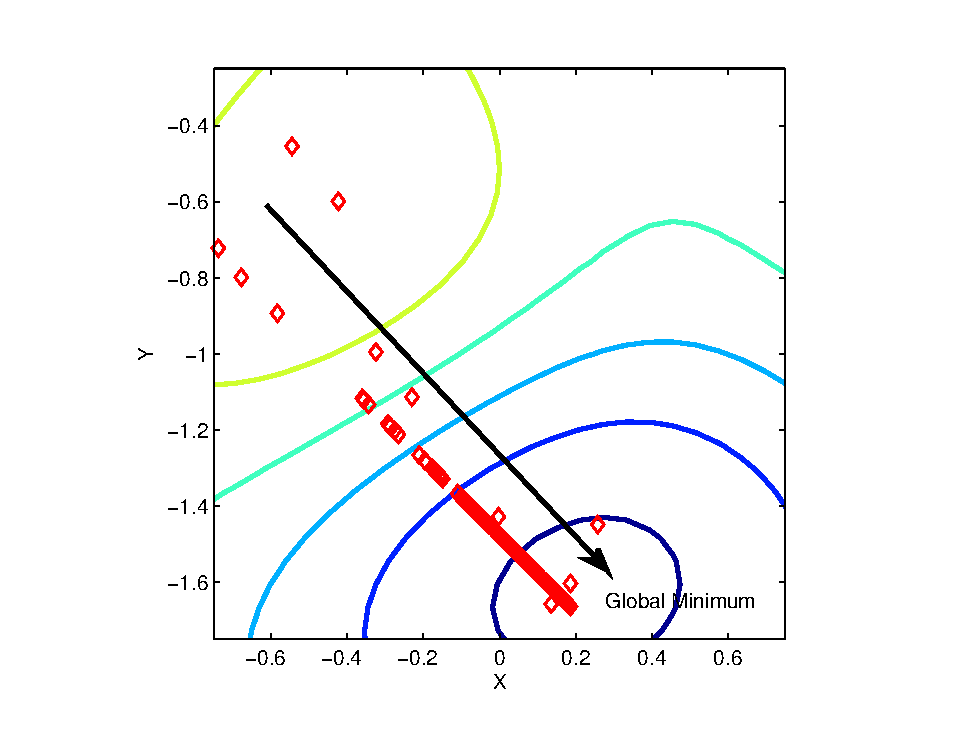
\includegraphics[width=0.8\textwidth]{./figures/peaks_descent.eps}
	\caption[MATLAB\textsuperscript{\textregistered} \textit{Peaks} Function
Minimization: Parametric Plot]{MATLAB\textsuperscript{\textregistered} \textit{Peaks}
Function
Minimization: Average Chromosome
	Parametric Plot}
	\label{fig:peaks_descent}
\end{figure}
%----------------------------

\subsubsection{Example 2: Rastrigin Function}
The Rastrigin function is a highly multimodal nonlinear function that is often used to
test global optimizers and specifically genetic algorithms. The Rastrigin function,
$f(\bm{x})$ is defined as
%----------------------------
\begin{equation}\label{eq:rastigrin}
f(\bm{x}) = \sum_{i=1}^{N}\Bigl[x_{i}^2-10\cos\bigl(2\pi x_i\bigr)+10\Bigr]
\end{equation}
%----------------------------
and the two dimensional case is plotted in Figure \ref{fig:rast_surf}. As illustrated in
Figure \ref{fig:rast_surf}, the two dimensional Rastrigin function is characterized by its
numerous local minima
and a global minimum at $(0,0)$.
%----------------------------
\begin{figure}[H]
	\centering
	\includegraphics[width=\textwidth]{./figures/rast_surf.eps}
	\caption{Two-Dimensional Rastrigin Function}
	\label{fig:rast_surf}
\end{figure}

\paragraph{Algorithm Setup and Initialization}
To find the global minimum of the the Rastrigin function, the HOG algorithm was
configured with a population size of 200 chromosomes. Each chromosome was seeded with
two alleles, $x_{1n}$ and $x_{2n}$, where $x_{1n}$ and $x_{2n}$ are continuous random
variables which are uniformly distributed over the feasible solution space,
$\left\{(x_1,x_2):-5.12\leq x_1\leq5.12,-5.12\leq x_2\leq5.12\right\}$. To
illustrate average performance metrics, the HOG algorithm was applied 50 times to
minimizing the cost function given in \eqref{eq:rastigrin}. For each trial, convergence
was defined as a lack of further improvement over 50 successive generations following a
minimum of 1000 generations. The remaining HOG algorithm parameters are summarized in
Table \ref{tbl:rast_setup}.
%----------------------------
\begin{table}[htbp]
 \begin{center}
 \caption[Rastrigin Function Minimization: Algorithm
Parameters]{Rastrigin Function Minimization: HOG Algorithm
Parameters}\label{tbl:rast_setup}
 \begin{tabular}{ l c }\toprule
 \textbf{Description} & \textbf{Value} \\ \midrule
Problem Dimension & 2 \\
Population Size & $200 \times 2$ \\
Feasible Solution Space & $-5.12\leq \{x_n,y_n\}\leq5.12$ \\
Probability of Crossover & $P_c = 0.2$ \\
Probability of Mutation & $P_m = 0.02$ \\
Selection Pressure & $\eta^+ = 1.1$\\ \bottomrule
\end{tabular}
\end{center}
\end{table}

\paragraph{Results}
In all 50 cases, the HOG algorithm successfully reached the global minimum. Figure
\ref{fig:rast_learning_curve} illustrates the average learning curve over all 50 runs of
the HOG algorithm when applied to the Rastrigin function.
%----------------------------
\begin{figure}[htbp]
	\centering
	\includegraphics[width=0.8\textwidth]{./figures/rast_learning_curve.eps}
	\caption{Rastrigin Function Minimization: Average Cost}
	\label{fig:rast_learning_curve}
\end{figure}
%----------------------------

Figure \ref{fig:rast_descent} shows a parametric plot of the Rastrigin function and plots
the average chromosome for each generation of a population for one of the 50
cases. As indicated by the arrows, the algorithm initially finds a local minima
adjacent to the global minimum. However, the average chromosome converges to the
global optimum value located at $(0,0)$.
%----------------------------
\begin{figure}[htbp]
	\centering
	\includegraphics[width=0.8\textwidth]{./figures/rast_descent.eps}
	\caption[Rastrigin Function Minimization: Parametric
Plot]{Rastrigin Function Minimization:
Average Chromosome Parametric
Plot}
	\label{fig:rast_descent}
\end{figure}

\subsubsection{Example 3: Rosenbrock Function}
The Rosenbrock function is a uni-modal non-linear function often used to evaluate the
performance of optimization algorithms. The Rosenbrock function, $f(\bm{x})$, is defined
as
%----------------------------
\begin{equation}\label{eq:rosenbrock}
f(\bm{x}) = \sum_{i=1}^{N-1}\Bigl[\bigl(1-x_i\bigr)^2+ 100 \bigl(x_{i+1} - x_i^2 \bigr)^2
\Bigr]
\end{equation}
%----------------------------
and the two dimensional case is plotted in Figure \ref{fig:rose_surf}. As illustrated in
Figure \ref{fig:rose_surf}, the two dimensional Rosenbrock function is characterized by
its long banana shaped valley with a global minimum at $(1,1)$.
\begin{figure}[htbp]
	\centering
	\includegraphics[width=\textwidth]{./figures/rose_surf.eps}
	\caption{Two-Dimensional Rosenbrock Function}
	\label{fig:rose_surf}
\end{figure}

\paragraph{Algorithm Setup and Initialization}
To find the global minimum of the the Rosenbrock function, the HOG algorithm was
configured with a population size of 200 chromosomes. The $n$th chromosome was seeded with
two alleles, $x_{1n}$ and $x_{2n}$, where $x_{1n}$ and $x_{2n}$ are continuous random
variables which are uniformly distributed over the feasible solution space,
$\left\{(x_1,x_2):-\pi\leq x_1 \leq\pi,-\pi\leq x_2\leq\pi\right\}$. To illustrate
average performance metrics, the HOG algorithm was applied 50 times to minimizing the cost
function given in \eqref{eq:rosenbrock}. For each trial, convergence was defined as a
lack of further improvement over 50 successive generations following a minimum of 1000
generations. The remaining HOG algorithm parameters are summarized in Table
\ref{tbl:rose_setup}.
%----------------------------
\begin{table}[htbp]
 \begin{center}
 \caption[Rosenbrock Function Minimization: Algorithm Parameters]{Rosenbrock Function
Minimization: HOG Algorithm Parameters}
 \label{tbl:rose_setup}
 \begin{tabular}{ l c }\toprule
 \textbf{Description} & \textbf{Value} \\ \midrule
Problem Dimension & 2 \\
Population Size & $200 \times 2$ \\
Feasible Solution Space & $-\pi\leq \{x_n,y_n\}\leq\pi$ \\
Probability of Crossover & $P_c = 0.2$ \\
Probability of Mutation & $P_m = 0.02$ \\
Selection Pressure & $\eta^+ = 1.1$\\ \bottomrule
\end{tabular}
\end{center}
\end{table}

\paragraph{Results}
In all 50 cases, the HOG algorithm successfully reached the global minimum. Figure
\ref{fig:rose_learning_curve} illustrates the average learning curve over all 50 runs of
the HOG algorithm when applied to the Rosenbrock function.
%----------------------------
\begin{figure}[htbp]
	\centering
	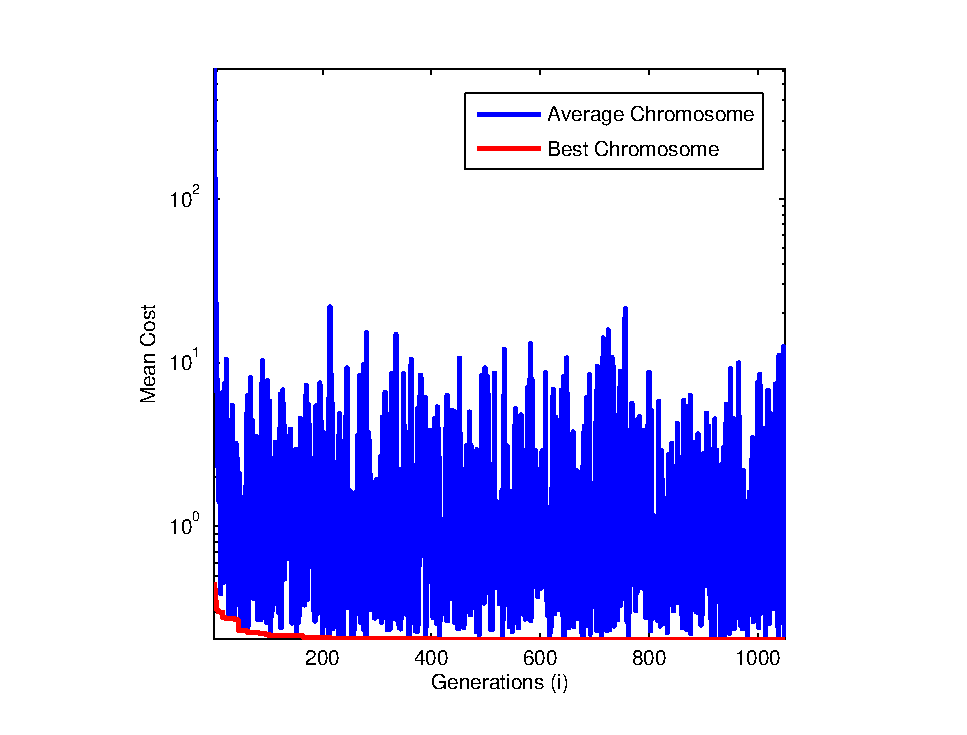
\includegraphics[width=0.8\textwidth]{./figures/rose_learning_curve.eps}
	\caption{Rosenbrock Function Minimization: Average Cost}
	\label{fig:rose_learning_curve}
\end{figure}
%----------------------------

Figure \ref{fig:rose_descent} shows a parametric plot of the Rosenbrock function
and plots the average chromosome for each generation of a population for one of the 50
cases. Figure \ref{fig:rose_descent} shows that the average chromosome converges to the
optimum value located at the global minimum $(1,1)$.
%----------------------------
\begin{figure}[htbp]
	\centering
	\includegraphics[width=0.8\textwidth]{./figures/rose_descent.eps}
	\caption[Rosenbrock Function Minimization: Parametric
	Plot]{Rosenbrock Function Minimization: Average Chromosome Parametric
	Plot}	
	\label{fig:rose_descent}
\end{figure}